\section{Implémentation des différentes versions} % (fold)
\label{sec:diff_rents_versions}
Dans cette partie, nous allons exposer les différentes versions parallèles du jeu de la vie que nous avons développées. Dans un premier temps, nous allons voir les différentes versions utilisant une mémoire partagée (section \ref{partagee}), puis les version \texttt{MPI} (section \ref{mpi}), utilisant d'abord des communications synchrones, puis des communications asynchrones, et enfin persistantes. Le code itère sur une boucle incrémentant une variable $loop$ qui indique combien de fois on a effectué l'actualisation du plateau. Nous nous intéressons surtout au code contenu dans cette boucle.

\subsection{Mémoire partagée}
\label{partagee}

\subsubsection{OpenMP}
\label{openmp}
\paragraph{Principe}
Dans le cas d'\texttt{OpenMP}, on va essayer de paralléliser les boucles de calcul du nombre de voisins et d'actualisation des cellules en fonction du nombre de voisins (figures \ref{boucle_voisins} et \ref{boucle_actualisation}), en distribuant les boucles sur un nombre prédéfini de threads. Pour cela, on spécifie simplement que l'on veut effectuer les boucles $for$ en parallèle avec l'instruction \ref{omp_parallel}, insérée juste avant les boucles. Dans le cas de l'exemple \ref{boucle_actualisation}, on veut calculer le nombre de cellules vivantes aussi. Pour ce faire, on effectue une réduction, employant l'opérateur addition sur la variable $num\_alive$. Le nombre de threads est fixé au tout début du programme, une fois les arguments passés en paramètre au programme lus. 

\begin{figure}[!ht]
\begin{lstlisting}
for (j = 1; j <= BS; j++) do
for (i = 1; i <= BS; i++) do
ngb( i, j ) =
cell( i-1, j-1 ) + cell( i, j-1 ) + cell( i+1, j-1 ) +
cell( i-1, j   ) +                  cell( i+1, j   ) +
cell( i-1, j+1 ) + cell( i, j+1 ) + cell( i+1, j+1 );
end do
end do
\end{lstlisting}
\caption{Boucle calculant le nombre de voisins}
\label{boucle_voisins}
\end{figure}


\begin{figure}[h!]
\begin{lstlisting}
for (j = 1; j <= BS; j++) do
for (i = 1; i <= BS; i++) do
if ( (ngb( i, j ) < 2) || (ngb( i, j ) > 3) ) 
cell(i, j) = 0;
else 
if ((ngb( i, j )) == 3)
cell(i, j) = 1;
fi
if (cell(i, j) == 1) 
num_alive ++;
fi
end do
end do
\end{lstlisting}
\caption{Boucle calculant l'état suivant des cellules et comptant le nombre de cellules vivantes}
\label{boucle_actualisation}
\end{figure}

\begin{figure}[h!]
\begin{lstlisting}
#pragma omp parallel for private(i,j)
\end{lstlisting}
\caption{Instruction \texttt{OpenMP}}
\label{omp_parallel}
\end{figure}

\paragraph{Pavage}
Nous avons implémenté une version \texttt{OpenMP} utilisant la notion de \emph{pavage}. Il s'agit de découper les boucles en $N$ plus petites boucles. Le but est de faire correspondre la taille des petites boucles avec la taille du cache, afin de bénéficier de ses performances. 

\subsubsection{\texttt{pthread}}
\label{pthread}

La version utilisant \texttt{pthread} découpe le plateau de jeu en plusieurs blocs. On associe un bloc à chaque thread du programme. Chaque thread calcule alors l'étape suivante pour son bloc. Ce découpage pose un problème de synchronisation entre les threads. En effet, si un thread modifie ses cellules alors qu'un autres n'a pas terminé de calculer son nombre de voisins, il est possible qu'il y ait des conflits sur les bords des blocs. La méthode retenue pour empêcher ces conflits est d'utiliser des barrières avec la bibliothèque \texttt{pthread}.

\subsection{Mémoire distribuée: \texttt{MPI}} % (fold)
\label{mpi}

Le but de cette version est de répartir les blocs de calcul sur plusieurs processeurs. Les processus ne contiennent dans cette version qu'un seul thread. On considère que les blocs sont tous de taille $m \times n$, $m$ le nombre de lignes et $n$ le nombre de colonnes. Des cases fantômes sont rajoutées tout autour du bloc, ce qui en fait des blocs de taille $(m+2) \times (n+2)$.

\paragraph{Communications synchrones}
Dans cette version, les communications sont synchrones. Pour cela, nous avons utilisé la fonction \emph{MPI\_Sendrecv}. \texttt{MPI} gère alors tout seul l'envoi et la réception sans créer de deadlocks. Nous aurions aussi pu, pour éviter les deadlocks, utiliser un système d'envoi des processus impairs puis pairs, ou encore faire en sorte qu'un processus reçoit avant d'envoyer (première version à préférer). 

\begin{figure}[!ht]
\begin{lstlisting}
Send(up,line[1])
Recv(up,line[0])
Send(down,line[m])
Recv(down,line[m+1])

for (j = 2; j < n; j++) do
	for (i = 2; i < m/2; i++) do
		calcul_nb_voisins(i,j);
	end do
end do

Waitall(1-4);

Send(left,column[1])
Recv(left,column[0])
Send(right,column[n-1])
Recv(right,column[n])

for (j = 2; j < n ; j++) do
	for (i = m/2; i <= m; i++) do
		calcul_nb_voisins(i,j);
	end do
	calcul_nb_voisins(1,j);
end do

Waitall(5-8);

for (j = 1; j <= n ; j+=n-1) do
	for (i = 1; i <= m; i++) do
		calcul_nb_voisins(i,j);
	end do
end do
\end{lstlisting}
\caption{Recouvrement des communications par des calculs}
\label{recouvrement}
\end{figure}


\paragraph{Communications asynchrones}
Pour bénéficier des communications asynchrones, il fallait recouvrir les communications par des calculs. Pour cela, nous effectuons d'abord la communication entre le processus situé au-dessus et celui en-dessous, pour ensuite communiquer avec les voisins de droite et de gauche. Nous pouvons alors recouvrir les communications avec le calcul des voisins (voir le code de la figure \ref{recouvrement}). 
Nous calculons la moîtié d'un bloc, sans les côtés, pendant la première partie des communications, puis le reste du bloc pendant la deuxième partie des communications, toujours sans les côtés de droite et de gauche (mais en faisant cette fois la ligne du haut et du bas, sans les extrêmes), pour enfin faire la colonne de droite et de gauche une fois que toutes les communications sont terminées. 
Dans le code de la figure \ref{recouvrement}, les $Send$ et $Recv$ sont tous asynchrones ($MPI\_Isend$ et $MPI\_Irecv$). On impose cependant une barrière permettant de s'assurer que ces communications sont finies (l. 12 et 27), lorsqu'on en a besoin pour la suite.

L'ordre des communications peut être résumé par le schéma de la figure \ref{fig:comm}. A noter que l'on envoie d'abord seulement les cellules que l'on connaît, ce qui constitue donc un envoie de taille $n$. Au deuxième tour de communications, l'envoi est de taille $m+2$.

\begin{figure}[!ht]
\centering
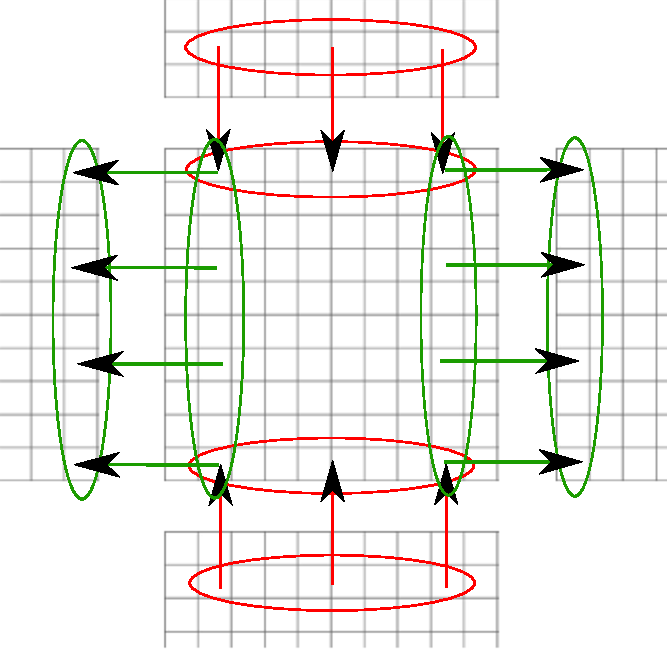
\includegraphics[width=0.6\textwidth]{comm.pdf}
\caption{Ordre des communications. Les rouges doivent se faire avant les vertes.}
\label{fig:comm}
\end{figure}

\paragraph{Communications persistantes}
Les communications sur la figure \ref{recouvrement}, des l. 1 à 4 et l. 14 à 17, sont remplacées par un simple $MPI\_Startall$, qui va lancer les requêtes, préparées à l'avance. De cette façon, les requêtes sont préparées dès le début du programme, une et une seule fois, et non pas à chaque tour de boucle de la variable $loop$. 